\section{Expériences/déploiements réalisés}
\label{sec:experiences_faites}

\begin{figure}[!t]
    \centering
    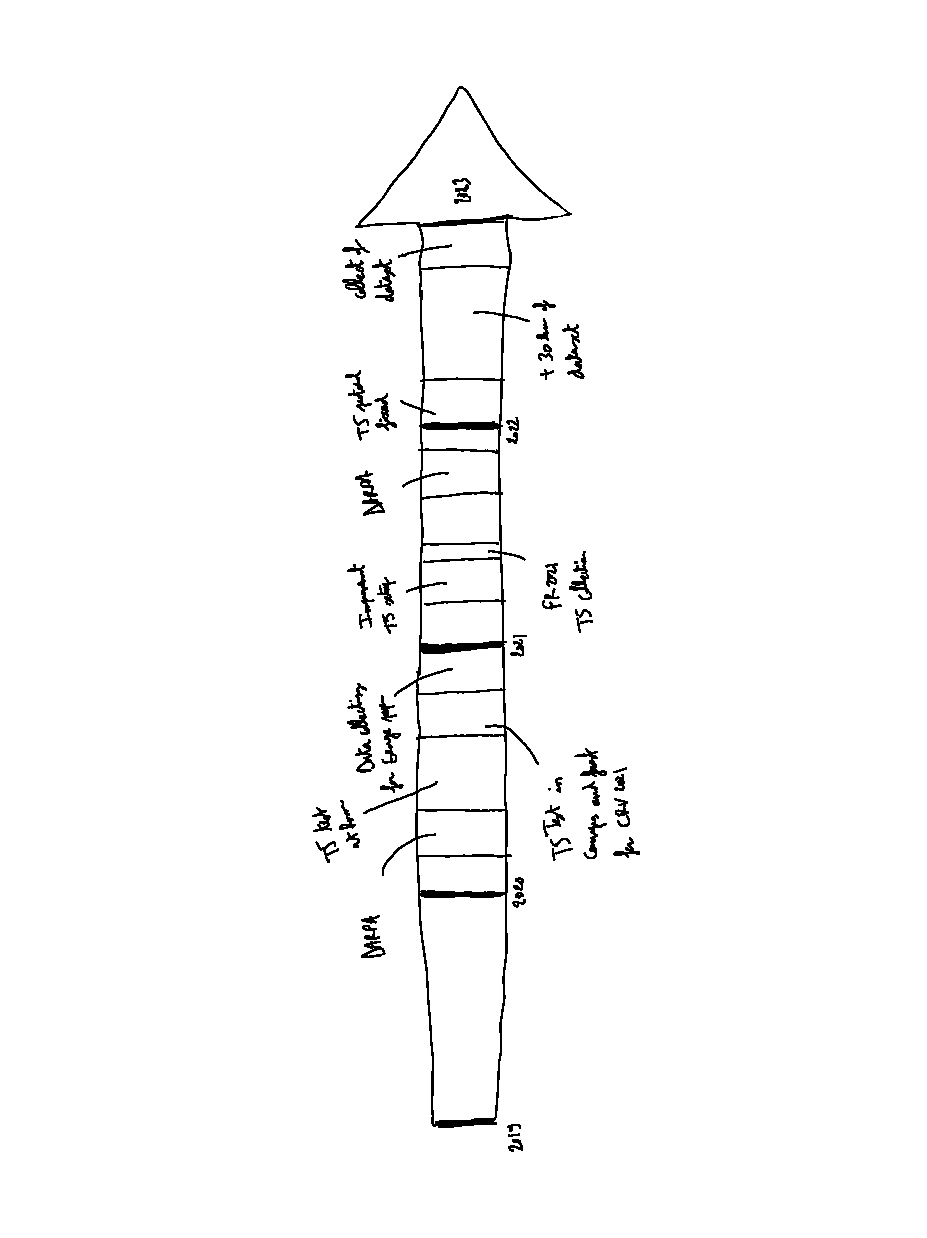
\includegraphics[width=\linewidth, angle=0, trim={0 0 0 0},clip]{figs/TS_timeline.pdf}
    \caption{Ligne de temps travaux TS}
    \label{fig:frise_exp}
\end{figure}

Au cours des quatre premières années de mon doctorat, j'ai effectué beaucoup de déploiements sur le terrain afin de tester et valider mes protocoles de déploiements, que ce soit pour mes stations totales robotiques, ou pour les plateformes robotiques que l'on utilise.
Cette section est destinée à détailler davantage les déploiements  illustrés sur la frise chronologique \autoref{fig:frise_exp}.
Les déploiements principaux ont été faits pour tester le système de stations totales dans différents types d'environnements.
Vient ensuite le DARPA challenge avec le déploiement de plateforme robotique dans des environnements souterrains.
Enfin, quelques déploiements annexes à mes recherches ont été réalisés en lien avec la prise de vérités terrains pour comparer des algorithmes de cartographie ou de contrôle.

\subsection{Stations totales robotiques}

La très grande majorité des déploiements avait pour but de  développer le système de stations totales robotiques.
Ces dernières ont été reçues au début de l'hiver 2020 et j'ai concrétisé le développement du code permettant de les faire fonctionner au printemps 2020.
Le système de collecte des données fut tout d'abord testé correctement en laboratoire,puis en environnement extérieur,sur le campus de l'université et en forêt de Montmorency, durant l'été et l'automne 2020.
Les données alors recueillies ont permis de rédiger le papier de CRV 2021.

À la suite de la publication de CRV 2021, de nouveau tests sur le campus et en forêt ont été réalisés au printemps 2021 afin d'améliorer le système d'acquisition des données. 
Le protocole de déploiement du système a été travaillé et finalisé entre octobre 2021 et février 2022 à la suite d'une bonne douzaine de déploiements.
Il se résume ainsi : si on utilise le système des stations totales pour un déploiement, on est sûr à 100\% d'avoir nos données, ce qui n'était pas le cas précédemment du fait de problèmes techniques ou d'une mauvaise utilisation des équipements.
 Trois expériences consécutives réussies sans problème pour l'acquisition des données ont validé le protocole.

 Le protocole stabilisé a permis la collecte du dataset pour le papier d'ICRA 2023 ( fin février 2022 jusqu'à mi-septembre 2022).
Cette collecte a été faite dans deux types d'environnements principaux, à savoir sur le campus de l'Université Laval en extérieur, mais aussi dans ses tunnels.
L'extérieur a été utilisé afin de pouvoir récolter des données \ac{GNSS} et de les comparer avec le système de stations totales.Mais là, il fut également possible d'accéder à des pylônes de calibration utilisée en géomatique, au positionnement relatif connu au millimètre près.La comparaison entre différentes méthodes de calibration extrinsèque fut ainsi aussi rendue possible.
Les tunnels ont été utilisés puisque des expériences de cartographie ont été menées pour un projet annexe de fin de maîtrise, et que, dans ce cas, des vérités terrains se révélaient nécessaires.
Deux plateformes robotiques ont été déployées, à savoir un Warthog de la compagnie ClearPath, et un HD2 de la compagnie SuperDroid.
Au total, le dataset se compose de 15 déploiements constitUtifs de 40 expériences,lesquelles totalisent plus de 32 kilomètres de trajectoires des plateformes robotiques.
Ce dataset est disponible en ligne. \href{https://github.com/norlab-ulaval/RTS_Extrinsic_Calibration/wiki/RTS-2022-Dataset}{ici}.

\subsection{DARPA}

Description DARPA competition, pourquoi relié à mes recherches

DARPA URBAN

DARPA FINALS

\subsection{Projets annexes en lien avec stations totales robotiques}

Projets annexes utilisant les stations totales, condition utilisation et pourquoi (amélioration algorithme)

Georges project

FR 2021 - teach-repeat

Matej project